\documentclass{ltjsarticle}

\usepackage{amsmath}
\usepackage{amssymb}
\usepackage{amsthm}
\usepackage{ mathrsfs }
\usepackage{enumerate}
\usepackage{bbm}
\usepackage{lipsum}
\usepackage{fancyhdr}
\usepackage{tikz-cd} 
\usetikzlibrary{graphs}
\usepackage{luatexja-ruby} 
\usepackage{graphicx} 
\graphicspath{ {./images/} }

\newtheorem{theorem}{定理}[section] 
\newtheorem{proposition}{Proposition}[section] 
\newtheorem{definition}{定義}[section] 
\newtheorem{problem}{問題}[section] 
\newtheorem{postulate}{公準}[section] 
\newtheorem{lemma}{Lemma}[section] 
\newtheorem{notation}{Notation}[section] 
\newtheorem{remark}{注釈}[section] 
\newtheorem{corollary}{系}[section] 
\newtheorem{terminology}{Terminology}[section] 
\newtheorem{example}{例}[section] 
\newtheorem{step}{手順} 
\newtheorem{solution}{解答}[section] 
\newtheorem{fact}{事実}[section] 


\DeclareMathOperator{\diam}{diam}
\DeclareMathOperator{\Gal}{Gal}
\DeclareMathOperator{\rank}{rank}
\DeclareMathOperator{\Hom}{Hom}
\DeclareMathOperator{\Dom}{Dom}
\DeclareMathOperator{\Ann}{Ann}
\DeclareMathOperator{\grad}{grad}
\DeclareMathOperator{\Span}{Span}
\DeclareMathOperator{\interior}{int}
\DeclareMathOperator{\ind}{ind}
\DeclareMathOperator{\supp}{supp}
\DeclareMathOperator{\ob}{ob}
\DeclareMathOperator{\Spec}{Spec}
\DeclareMathOperator{\MaxSpec}{MaxSpec}
\DeclareMathOperator{\PreSh}{PreSh}
\DeclareMathOperator{\Sh}{Sh}
\DeclareMathOperator{\Fun}{Fun}
\DeclareMathOperator{\Ext}{Ext}
\DeclareMathOperator{\Aut}{Aut}
\DeclareMathOperator{\Ker}{Ker}
\DeclareMathOperator{\Image}{Im}
\DeclareMathOperator{\Coker}{Coker}
\DeclareMathOperator{\id}{id}
\DeclareMathOperator{\Mod}{Mod}
\DeclareMathOperator{\QCoh}{QCoh}
\DeclareMathOperator{\Coh}{Coh}
%\newcommand*{\name}[\num_arguments][default values]{{\color{#1}\Large #2}}
\newcommand*{\multivar}[2]{{#1_1,\cdots,#1_{#2}}}
\newcommand*{\localization}[2]{#1_{\mathfrak{#2}}}
\newcommand*{\ringedspacemorph}[1]{(#1,#1^{\#})}
\newcommand*{\sheaf}[2]{(#1,{\mathcal{#2}}_{#1})}
\newcommand{\fib}[1]{%
  \mathbin{\mathop{\times}\limits_{#1}}%
}
\newcommand{\tens}[1]{%
  \mathbin{\mathop{\otimes}\displaylimits_{#1}}%
}
\title{ボン補習校高校数学}
\author{}
\date{}

\begin{document}

\maketitle
\section{微分積分}
変化のことについて、変化のようが時間とともに変化することについて。
\begin{problem}
電車が$100$キロメートルを進むのに$1.25$時間かかりました。電車の速度は時速何キロですか。
\end{problem}
\begin{proof}[解答]
\begin{equation*}
100\div 1.25 = 80
\end{equation*}
よって時速$80$キロメートルが答え。
\end{proof}

この問題をよく考えてみましょう。$100$メートルというのは位置の変化です。最初の場所から$1.25$時間あとにいる場所への距離のこと。$1.25$時間とはこの変化にかかった時間です。時速$80$キロメートルというのは１時間でどのくらい位置が変化するのかということを示します。よって上の問題は次のように言い換えることができます。
\begin{equation*}
\text{時速$80$キロメートルで$1.25$時間移動すると$100$キロメートル進める。}
\end{equation*}

電車の位置を$x$、現在の時間を$t$とします。数学や物理ではこれらの変化のことを

\begin{equation*}
\Delta x,\Delta t
\end{equation*}
などと書きます。上の問題では
\begin{equation*}
\Delta x = 100, \Delta t = 1.25
\end{equation*}
となります。$\Delta$は英語の「Difference」の頭文字$D$のギリシャ文字$\Delta$から取られました。

変化の割合について知ることで実際に起こった変化を知ることができます。この例では変化の割合は常に同じ（一定）でしたが、時間によって変化の割合が変わることもあります。
\begin{example}
人口の変化を考えてみましょう。大人の数が多ければ多いほど、生まれてくる子供の数も多くなります（比例する）。また、事故や病気で大人が亡くなることもあるでしょう。この場合では電車の時速とは違い、変化の割合は常に変わります。これを式にすると次のようになります。
\begin{equation*}
{\frac {\Delta\text{人口}}{\Delta\text{時間}}} = \text{比例定数}\times\text{時間$t$での大人の数}
\end{equation*}
\end{example}

\begin{example}
ある物を持ち上げて静かに落とした時のことを考えます。より高いところから落とすと地面に着く前の速度はより速くなります。これは地面につくまでより時間がかかっていることが原因です。また速度が上がれば押しのける空気の量も増えます。この空気の量を空気抵抗と呼びます。言い換えると空気抵抗は速度に比例する。よってこれは次のようにかけます。
\begin{equation*}
{\frac {\Delta\text{速度}}{\Delta\text{時間}}} =\text{時間$t$での速度の変化}-  \text{比例定数}\times\text{時間$t$での空気抵抗}
\end{equation*}
\end{example}

上の例の場合、速度は時間が進めば進むほど変わっていきます。より時間が空気抵抗に与える影響を少なくし、空気抵抗を正確に測るためには変化の時間を小さくする必要があります。数学的にこれは
\begin{equation*}
\lim_{\Delta t\to0}{\frac {\Delta\text{速度}}{\Delta\text{時間}}} ={\frac {d\text{速度}}{d\text{時間}}} 
\end{equation*}
というふうに書きます。変化の割合が一定の場合は最初の電車の例のように簡単に実際の変化が計算できました。微分積分では時間によって変化の割合が変わっても、変化を計算するにはどうすればよいかを勉強します。
\section{グラフ理論}
グラフ理論とは次のような形の図形（グラフ）を考える学問です。
\begin{center}
\begin{figure}[h]
	\centering
    
\includegraphics[scale=0.6]{graph}
    \caption{グラフの例}
    \label{fig:my_label}
\end{figure}
\end{center}
Googleなどの検索エンジンやSNSのように、欲しい情報を探すことや、情報を人それぞれによって整理して提供することはプログラミングにおいてとても重要な分野です。効率よく探す方法を見つけることも大事ですが、最初から整理整頓されていれば欲しい情報をより速く見つけることができます。そのようなデータを整理する方法を探すのがグラフ理論です。次のグラフを見てみましょう。
\begin{center}
\begin{figure}[h]
	\centering
    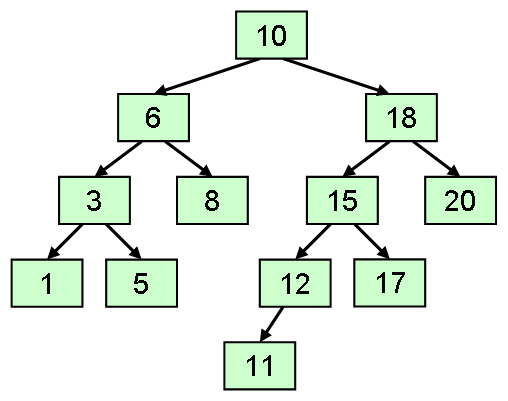
\includegraphics[scale=0.4]{binarytree}
    \caption{\ltjruby{二分探索木}{にぶんたんさくぎ}}
    \label{fig:my_label}
\end{figure}
\end{center}
ある数字の左下にはそれよりも小さい数字、右下にはそれよりも大きい数字が置かれています。このようにデータを整理することで一番小さい数は$1$で大きい数は$20$であることがわかります。これはコンピューターにもとても使いやすい形でプログラミングの世界では広く使われています。また下の図のようにソーシャルメディアにおいて友達関係を次のように表すことで情報を整理することもできます。
\begin{center}
\begin{figure}[h]
	\centering
    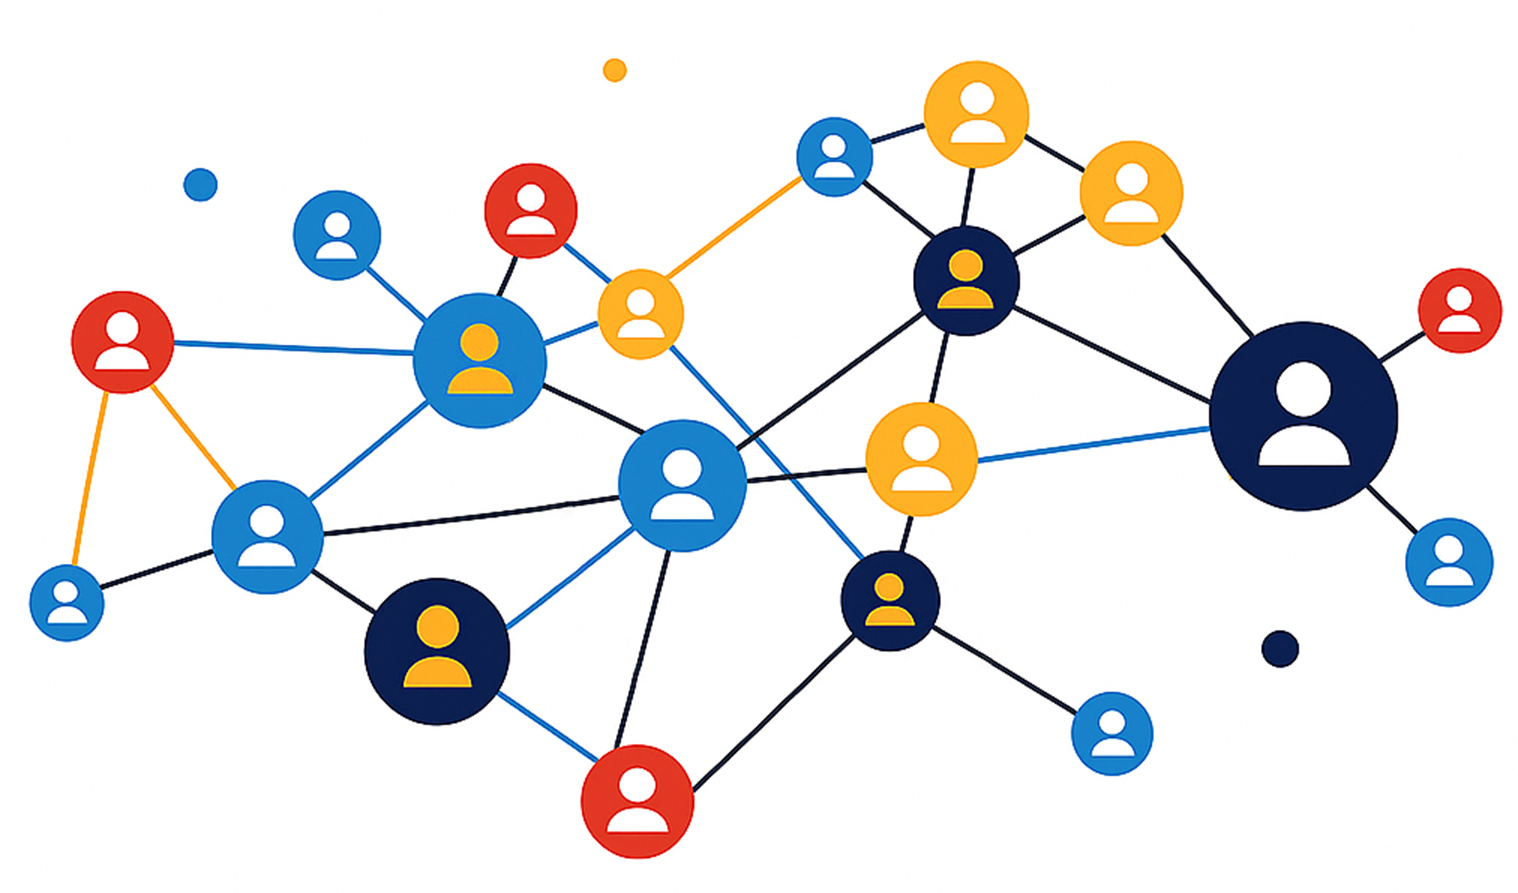
\includegraphics[scale=0.1]{followers}
    \caption{SNSでの応用}
    \label{fig:my_label}
\end{figure}
\end{center}
\section{整数論}
整数論ではあまりのある割り算を中心に授業を行います。あまりのある$7$で割った割り算を考えてみましょう。整数$a,b$を$7$で割った時の余りが等しい時これを、
\begin{equation*}
a\equiv b\mod{7}
\end{equation*}
と書きます。例えば
\begin{equation*}
2\equiv 9\mod{7},14\equiv 0\mod{7},3\equiv 38\mod{7}
\end{equation*}
となります。この計算は足し算と掛け算にも対応しています。例えば、
\begin{equation*}
2+ 3 = 5, 9 + 38 = 47 = 7\times 6 + 5
\end{equation*}
よって
\begin{equation*}
2+3 \equiv 9+38 \mod{7}
\end{equation*}
また
\begin{equation*}
2\times 3 = 6, 9 \times 38 = 342 = 7 * 48+6
\end{equation*}
よって
\begin{equation*}
2\times3 \equiv 9\times38 \mod{7}
\end{equation*}
このようにして整数は次の７つのものに分類されます
\begin{equation*}
\{\text{$7$で割り切れる数}\},\{\text{$7$で割って$1$余る数}\},\cdots\{\text{$7$で割って$6$余る数}\}
\end{equation*}
さっき見たように、この分類は足し算と掛け算にも対応しています。どのようにしてこの考え方が役に立つのでしょうか。
数学は物理、化学、また生物のような自然科学とは少し異なった性質を持ちます。自然科学では実際に存在するものを研究します。存在しないものを研究しても意味がないですよね。では数学では何を持ってある概念が存在するとしているのでしょうか。数学において存在するとは文字と整数で表すことができることです。例えば、有理数は
\begin{equation*}
{\frac 2 3},{\frac {13} 5}
\end{equation*}
のように二つの整数で表すことができます。また直線や二次関数などは
\begin{equation*}
y = 5x+3, y = 3x^2+3x-7
\end{equation*}
のように整数と二つの文字$x,y$で表されます。では無理数や虚数はどのようにして表されるのでしょうか。数字と文字そしてそこにあまりを考えた分類をすることでこれらの数を表すことができます。簡単にいうと
\begin{enumerate}[ステップ1：]
\item 数字と文字を使ってとても大きな数の集まりを作る。
\item 余りを考えた計算でいらないものを除去していく。
\end{enumerate}
というようなことをします。この単元ではこの方法でいかにして無理数や虚数が作られるのかを学びます。
\section{図形}

平面図形では日本の高校数学に習います。最初に三角形の五心を学びます。これは三角形とそれに関わる円の中心の関係についての分野です。まずはそのうちの三つの円について見てみましょう。

\begin{center}
\begin{figure}[h]
	\centering
    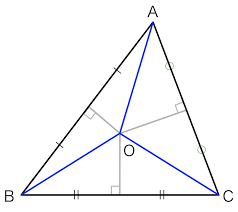
\includegraphics[scale=0.4]{outercircle}
    \caption{三角形の外心}
    \label{fig:my_label}
    三角形のそれぞれの辺の垂直二等分線の交点。
\end{figure}
\end{center}
\begin{center}
\begin{figure}[h]
	\centering
    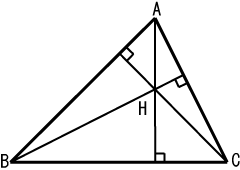
\includegraphics[scale=0.4]{perpendicularcircle}
    \caption{三角形の垂心}
    \label{fig:my_label}
    三角形のそれぞれの頂点から向かい合う線に垂直に引いた線の交点。
\end{figure}
\end{center}
\begin{center}
\begin{figure}[h]
	\centering
    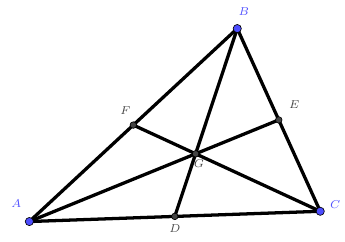
\includegraphics[scale=0.4]{barycenter}
    \caption{三角形の重心}
    \label{fig:my_label}
    三角形のそれぞれの頂点から向かい合う線の中点に引いた線の交点。
\end{figure}
\end{center}
これら三つの点について次のことが成り立ちます。
\begin{figure}[h]
	\centering
    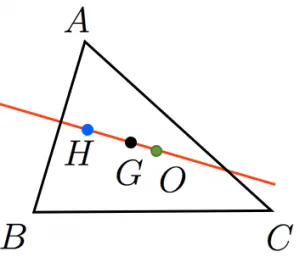
\includegraphics[scale=0.4]{eulerline}
    \caption{三角形のオイラー線}
    \label{fig:my_label}
    $H$を垂心、$G$を重心そして$O$を外心とするとこれらは一つの直線に乗る。
\end{figure}

このような定理の証明には三角比やベクトルを使ったものがありますが、それらを使わずにすむ美しい証明をたくさん紹介できればよいと考えています。また発展分野として双極幾何学というのを予定しています。平面幾何は平らな世界の幾何学。われわれのご先祖さまたちが平地で農作をするために作った学問です。それに対して双極幾何学は宇宙の幾何学、アインシュタインが相対性理論を作った元になった幾何学を紹介したいと考えています。
\begin{center}
\begin{figure}[h]
	\centering
    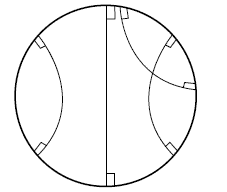
\includegraphics[scale=0.4]{poincare}
    \caption{ポアンカレディスクモデル}
    \label{fig:my_label}
    普通の幾何学とは違い、この双極幾何のモデルでは直線は円に対して垂直な弧となる。
\end{figure}
\end{center}
\end{document}